\subsection{Decision Tree}
\label{sec:tree}

%Decision tree algorithm has been widely used in ML problems. It has 
%been proven to be efficient in classification. 
As a first step, a simple classification tree was generated from the 
training data. 
The tree was built using CART (Classification and Regression Trees) 
algorithm~\cite{CART}. 
CART constructs a binary tree, where each node has two output leaf 
nodes. 
Gini gain selection was used for the splitting. The final tree graph 
is presented in the Figure~\ref{fig:tree}.
%The simple classification tree shows a $94\%$ sensitivity level, see 
%Table~\ref{tbl:res}.
See Table~\ref{tbl:res} for the performance results.

As a next step, to improve performance of the model, we tried 
Bootstrap Aggregation (Bagging) ~\cite{Bagging} on trees. 
Bagging algorithm creates subsets of data and trains decision trees 
on those subsets. 
It has been shown in that such methodology can 
effectively improve the stability of the algorithm ~\cite{Stability} 
and avoid 
overfitting~\cite{Overfitting}.
To decide on the number of trees for the Bagging algorithm, three 
performance measures were analysed: (1) sensitivity, (2) training 
time and (3) OOB. Figure~\ref{fig:tree_graph} shows the trade-off 
between the number of trees and three measures listed above.
%The sensitivity increases from $94\%$ for the simple classification 
%tree to $98\%$ for $13$ and more trees. 
%There is a decrease in sensitivity for models with even number of 
%trees in comparison with odd number of trees. 
%As number of trees grows, we can find a 
%notable increment in the training time. 
%When the number of trees increases to $10$, the OOB error 
%reaches $0.05$.

%\begin{enumerate}
%	\item When the number of bagging trees is $5$, the sensitivity 
%	reaches $96\%$ percent; when 
%	the number of trees increases to $7$, the sensitivity reaches 
%	$97\%$ percent; when the number of trees increase to $13$ or 
%	more, 
%	the sensitivity can reach about $98\%$ but can not stably stay 
%	above $98\%$
%	(both calculated by mean of 20 trials).
%	The result also shows a little decrease in sensitivity of even 
%	tree number
%	models compared with odd tree number models. 
%	%%%%%%%%%%%%5
%	\item 
%%Training time is also necessary to evaluate when we use our model 
%%in 
%%a clinical environment. 
%	As number of trees grows, we can find a 
%	notable increment in the training time. When the number of 
%	trees is $7$, training time per patient reaches $0.01$s.
%	%%%%%%%%%%%%%%
%	\item The third evaluation method is called OOB 
%	(Out-Of-Bag)~\cite{OOB} error. 
%	After generating the classifier ($S$ trees), for each $(X_i, 
%	y_i)$ in the original splitted training set (for example, $T$-th 
%	training set), select all $T_k$ that do not include $(X_i, y_i)$. 
%	This subset is a set of boosttrap datasets that do not contain 
%	specific records from the original dataset. 
%	This set is called an Out-of-bag example. 
%	There are $n$ such subsets (one for each data record in the 
%	original data set $T$). OOB classifier is the aggregation of 
%	votes only over $T_k$, such that it does not contain $(X_i,y_i)$. 
%	Then Out-of-bag error is the prediction error rate of the 
%	out-of-bag classifier on the training 
%	set. When the number of trees increases to $10$, the OOB error 
%	reaches $0.05$.
%\end{enumerate}

\paragraph{Implementation.}
We used the MATLAB class \textit{TreeBagger}, from Statistics and 
Machine Learning Toolbox~\cite{treebagger_matlab} to generate our 
classifiers. 
See MATLAB code for more details.
%The following settings were used: 
%\texttt{Method} $\to$ \texttt{classification}; To obtain the simple 
%decision tree model: \texttt{trees 
%number} $\to$ $1$; 
%To perform bagging: \texttt{trees number} $\to$ 
%$\{1,3,5,\ldots,25\}$; 
%To get the relationship between OOB error and the number of trees:
%\texttt{OOBPredictorImportance} $\to$ \texttt{On}. 

\begin{figure}[t]
	\centering
	\begin{subfigure}{.7\textwidth}
		\centering
		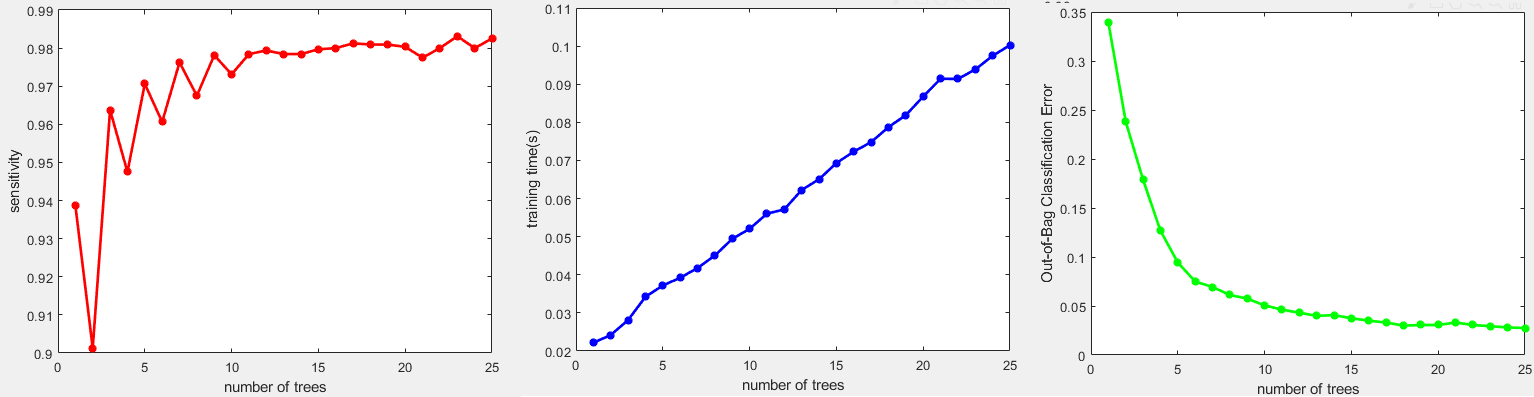
\includegraphics[width=.95\textwidth]{figures/tree_graph.png}
		\caption{Tree Estimations: Trade-off between the number of 
		trees 
			and (left subplot) Sensitivity, (middle subplot) training 
			time, 
			(right subplot) OOB.}
		\label{fig:tree_graph}
	\end{subfigure}%
	\begin{subfigure}{.35\textwidth}
	\centering
	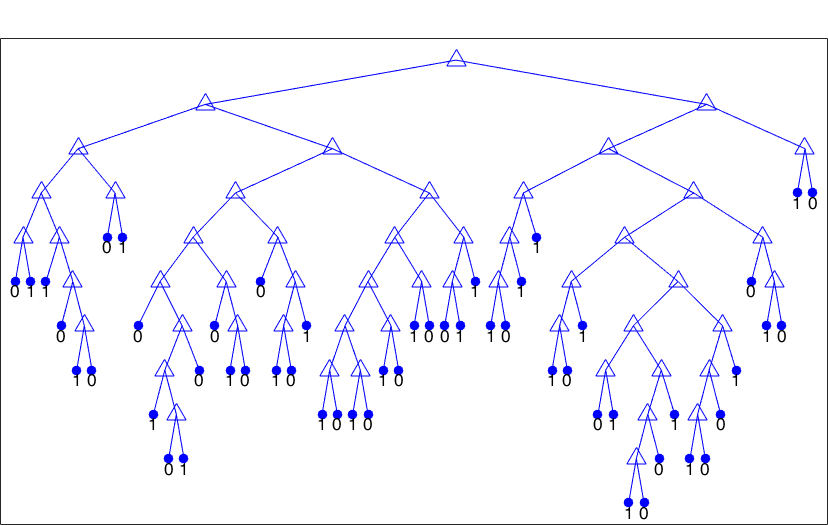
\includegraphics[width=.9\textwidth]{figures/tree.png}
	\caption{Learned tree graph structure.}
	\label{fig:tree}
	\end{subfigure}
	\caption{Decision tree plots}
	\label{fig:t}
\end{figure}

%\begin{figure}[t]
%	\centering
%	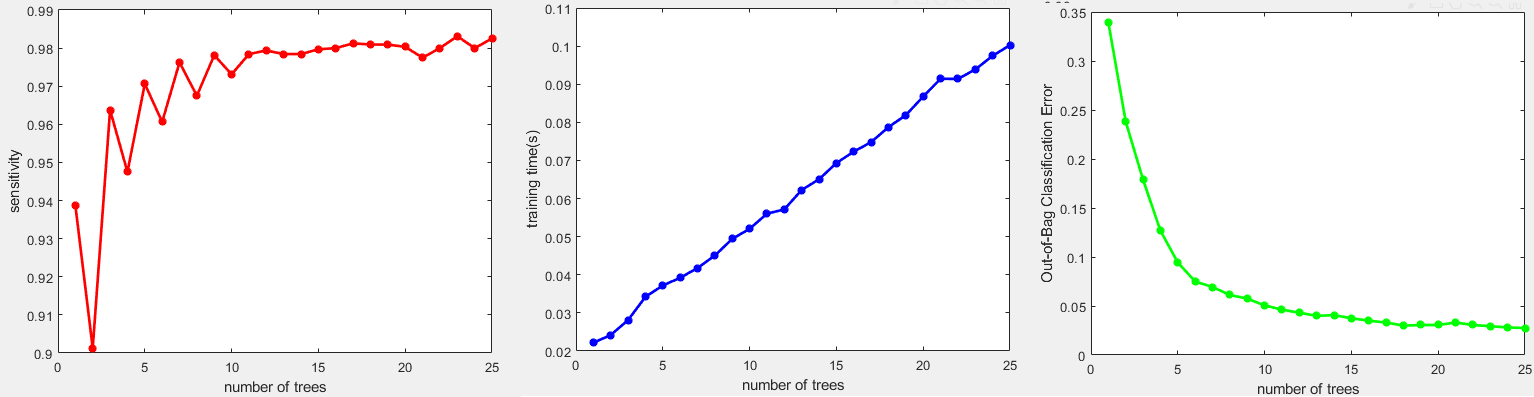
\includegraphics[width=1\textwidth]{figures/tree_graph.png}
%	\caption{Tree Estimations: Trade-off between the number of trees 
%		and (left subplot) Sensitivity, (middle subplot) training 
%time, 
%		(right subplot) OOB.}
%	\label{fig:tree_graph}
%\end{figure}
%\begin{figure}[t]
%	\centering
%	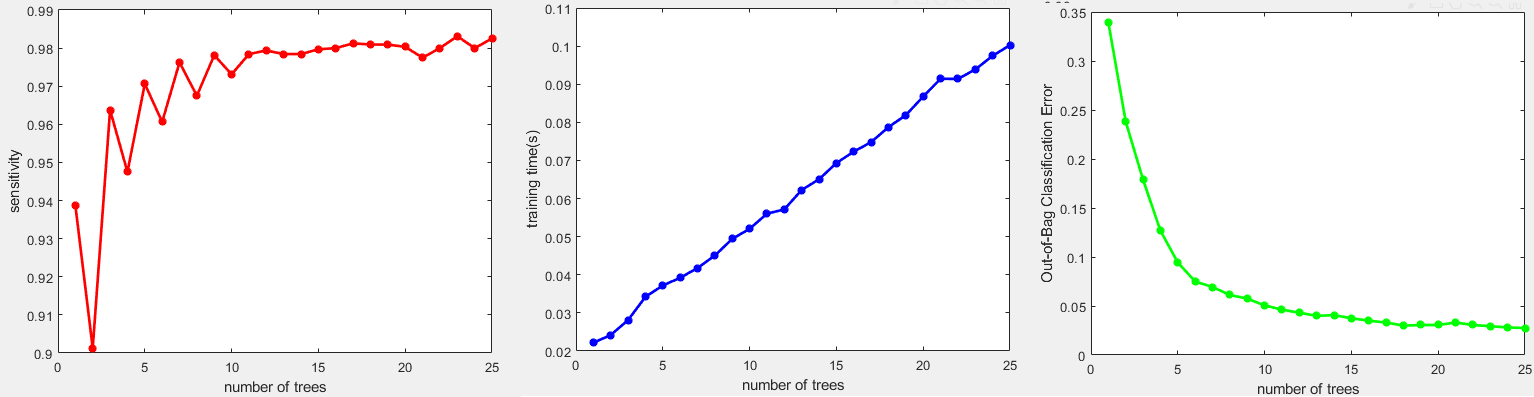
\includegraphics[width=1\textwidth]{figures/tree_graph.png}
%	\caption{Tree Estimations: Trade-off between the number of trees 
%	and (left subplot) Sensitivity, (middle subplot) training time, 
%	(right subplot) OOB.}
%	\label{fig:tree_graph}
%\end{figure}